\section{ Limites et Etudes Complémentaires}
\label{sec:Ch4}

%%%%%%%%%%%%%%%%%%%%%%%%%%%%%%%%%%%% SUBSECTION 1
\subsection{Limites}
\label{sec:Ch4.1}

Tout d'abord Breukels ne prend en compte que le diamètre et la cambrure maximal d'un profil, \textbf{la position de la cambrure maximale d'un profil n'est donc pas prise en compte}. \\

Ensuite, l'étude réalisée \textbf{ne fait pas intervenir de critère de stabilité.} Il sera sujet par suite d'une telle étude avec les résultats obtenus dans ce papier.\\

De plus, le choix de la fonction objective pour la recherche d'un optimum (moyenne pondérée par une Gaussienne) est peu justifiée. Connaître la valeurs d'un angle d'attaque pour lequel on souhaite optimiser une fonction ( finesse, stabilité, portance...) permettrait d'avoir un résultat plus pertinant. \textbf{Mesurer les angles d'attaques principaux lors des essais kite, peut-être avec l'extended Karmann Filter (EKF)} fournit par Kite Power, permettrait de répondre à ce problème. Le choix de sigma et alpha center dans la Gaussienne sont, eux aussi, criticables.\\

Finalement les fonctions d'optimisation d'Aerosandbox ne sont pas applicables à la VSM. Elles sont cependant utilisées pour optimiser la fonction de Breukels (2 paramètres). \\
Aerosandbox peut aussi représenter et optimiser les profils avec 10 paramètres (Kulfan parameters). Ce n'est pas le sujet de ce papier, cependant c'est une façon différente d'aborder le problème. 

\begin{figure}[H]
    \centering
    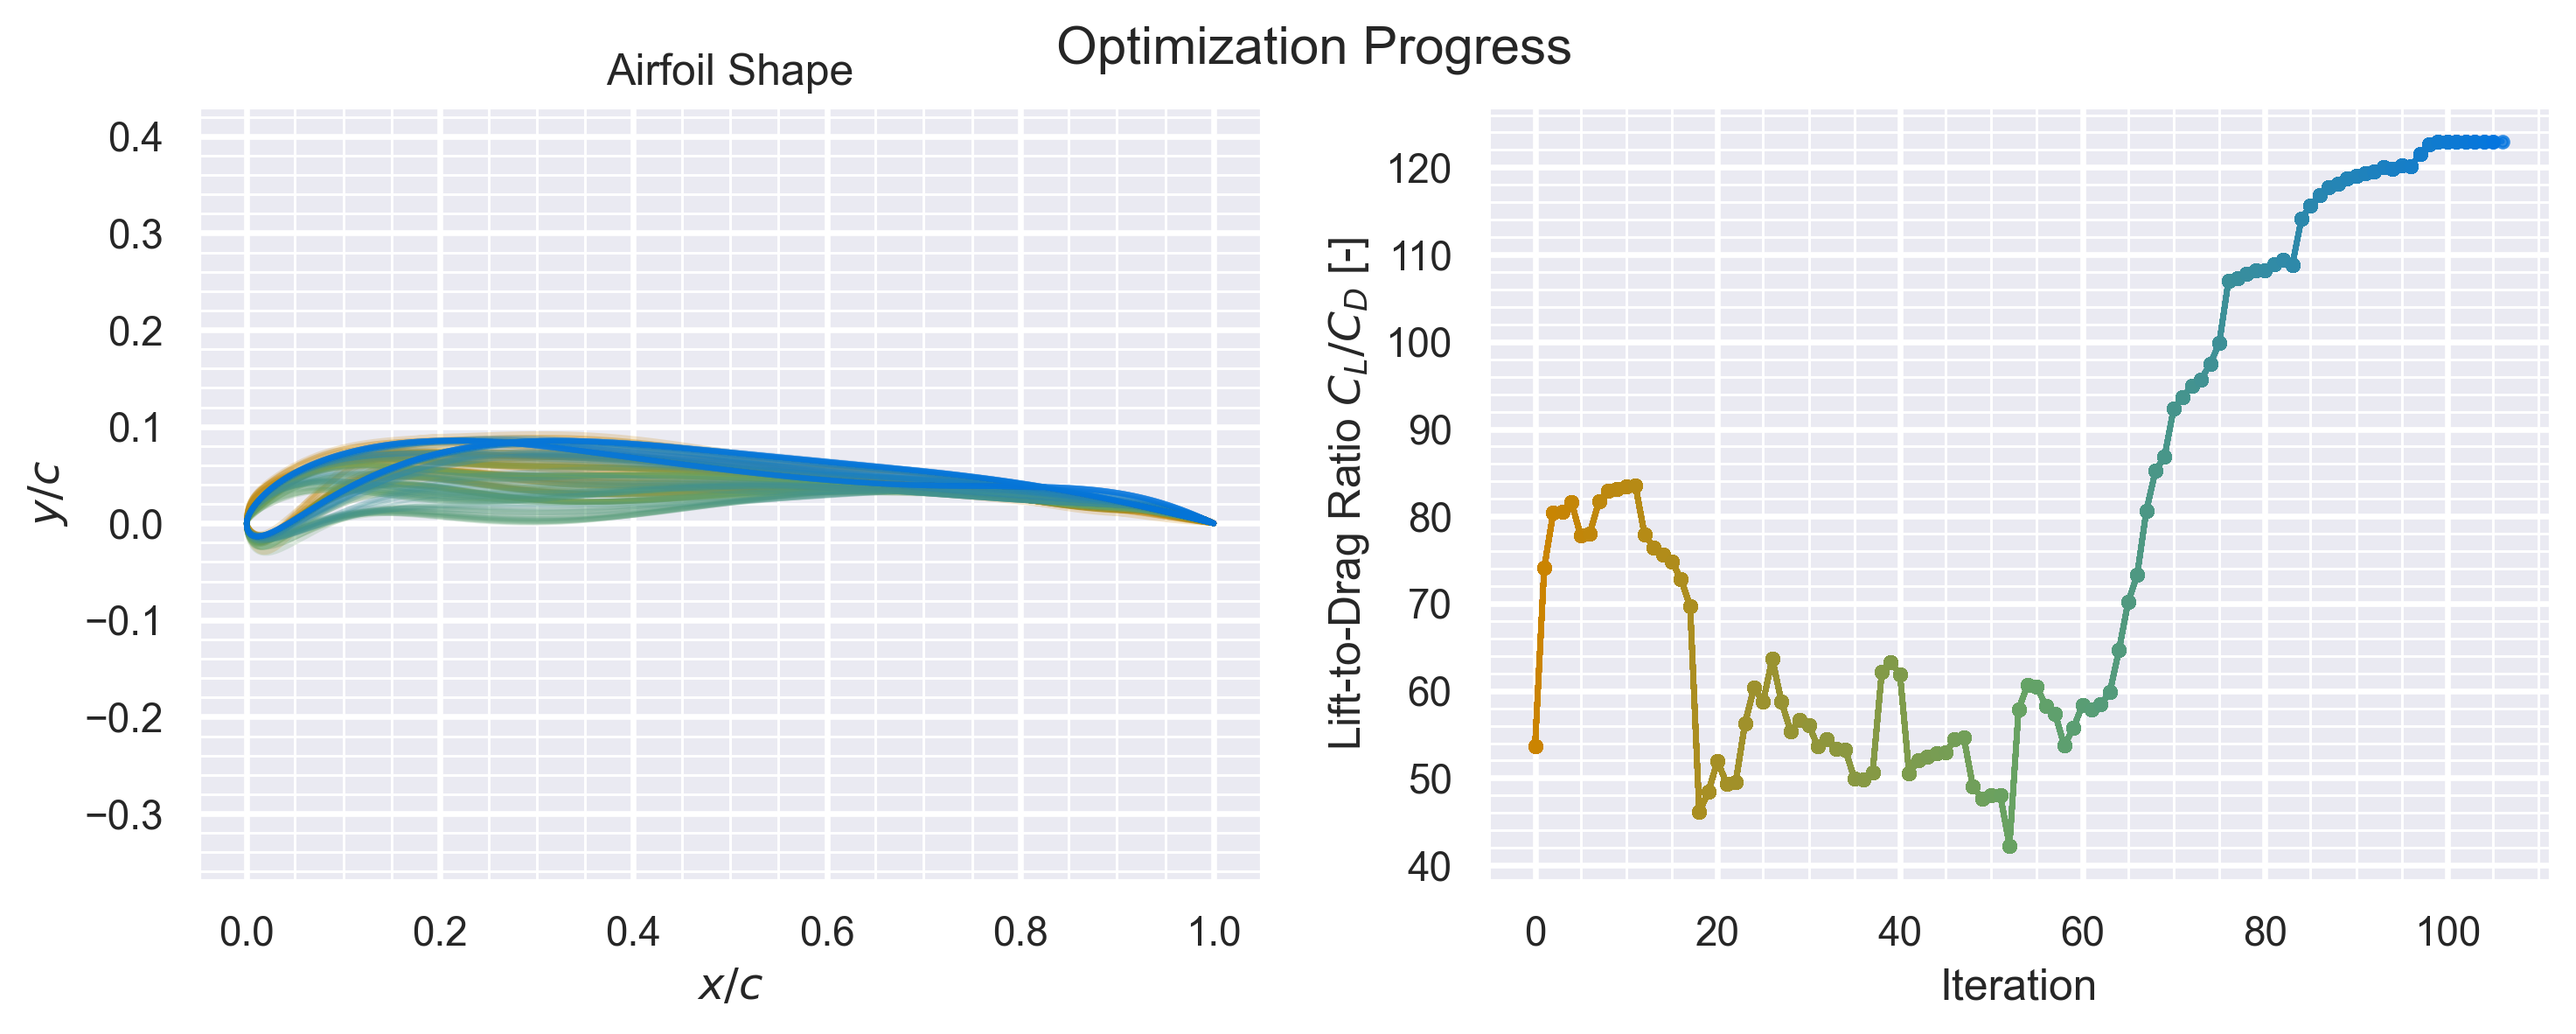
\includegraphics[width=0.5\textwidth]{Pics/optim neuralfoil.png}  
    \caption{Optimisation réalisée avec Aerosandbox sur des profils dis "de Kulfan"}
    \label{fig:kulfan}
\end{figure}

%%%%%%%%%%%%%%%%%%%%%%%%%%%%%%%%%%%% SUBSECTION 2
\subsection{Etudes complémentaires}
\label{sec:Ch4.2}

\begin{itemize}
    \item Comparer sur NeuralFoil et/ou XFoil le profil actuel d’une VG avec le profil optimisé trouvé par OptimXBreukels
    \item Comparer aussi le Cm des 2 profils -> potentiellement conclure sur un profil + performant + stable ?
    \item Créer une base de données d'airfoils polars grâce à Aerosandbox ? qui prend en compte les 3 paramètres (diameter, x depth et depth) et les faire tourner en 2D et ou sur la VSM pour trouver le profil optimal
    \item Faire un chapitre de comparaison des 10m2 classiques vs Hybrid avec profil à caisson, quantifier l'impact de la double peau
\end{itemize}
